\chapter{Felhasználói dokumentáció}
A \textit{DiagramQuery} első sorban lehetőséget biztosít egy Oracle SQL adatbázishoz való kapcsolódáshoz, illetve
eme adatbázison lekérdezések, szkriptek végrehajtására, továbbá diagramok létrehozására ezen lekérdezések
segítségével.
A kapcsolatokat tartalmazó adatokat el is lehet menteni (valamint lehetőség van kézzel leírni,
ez kifejtésre kerül az első szekcióban.), illetve betölteni egy .xml formátumú fájlból.

A kapcsolat felépítése után juthatunk a fő ablakba, itt lehetőség van a fentebb említett SQL lekérdezések végrehajtására, 
azonkívül PL/SQL szkriptek futtatására,
illetve diagramokat is itt lehet készíteni, ennek részletezése a 2.3.-ban történik meg.

\section{Telepítés és beállítás}
A \textit{DiagramQuery} telepítése nem szükséges, ám a lemezen található minden állomány szükséges a futásához,
így futtatáshoz másoljon át minden fájlt, és futtassa a \textit{DiagramQuery.exe}-t.
Windows 10 alatt lett tesztelve, a program bármilyen rendszeren képes megfelelően működni ahol a
Windows 10 is elfut alkalmas módon.

Érdemes megjegyezni, hogy a DiagramQuery Qt keretrendszerben lett megírva. Ez azt jelenti, hogy nem csak Windowson lehet
futtatni fordítás után, hanem bármin amin Qt és OCI elérhető. Linuxon is tesztelve lett, és helyesen működik. A program telepítése
forráskódból:
\begin{enumerate}
  \item Qt 5.6, vagy frissebb letöltése és telepítése.
  \item Oracle Instant Client letöltése, valamint telepítése (Oracle oldalán elérhető, regisztrációhoz kötött).
  \item Qt OCI pluginjának fordítása.
  \item Utolsó lépésként egyszerűen fordítható a program, immáron működőképes kell legyen.
\end{enumerate}

Lehetőség van későbbi fejlesztések során további adatbázis-kezelők hozzáadására a forráskód birtokában, azonban ekkor
manuálisan kell telepíteni az előbb leírtak szerint.
Telepítés után lehetőség van manuálisan létrehozni kapcsolatokat. Ha ezt kívánja tenni, akkor hozzon létre egy
\textit{Connections} mappát a futtatható állomány könyvtárába, és hozzon létre egy .xml kiterjesztésű fájlt a kívánt névvel.

Egy példa a fájlra:

\begin{lstlisting}
  <?xml version="1.0" encoding="UTF-8"?>
  <Connection name="Elte">
      <host>aramis.inf.elte.hu</host>
      <port>1521</port>
      <service>eszakigrid97</service>
      <username>A8UZ7T</username>
  </Connection>
\end{lstlisting}

A fájl felépítése a következő legyen:
\begin{itemize}
  \item A második (és hetedik) sorhoz hasonlóan \textbf{Connection} címkék között legyen elhelyezve az egész kód, illetve legyen a
  nyitócímkének egy attribútuma: name, a kapcsolat nevével,
  \item \textbf{host} címkék között a kapcsolat címe legyen a harmadik sorban látható módon,
  \item \textbf{port} címkék között legyen megadva a kapcsolat portja úgy, ahogy a negyedik sorban látható,
  \item \textbf{service} címkék között legyen a szerviz neve az ötödik sorhoz hasonlóan,
  \item illetve \textbf{username} címkék között a bejelentkezéshez szükséges felhasználónév ugyanúgy mint a hatodik sorban.
\end{itemize}
Ha valamelyik mezőt nem szeretné eltárolni, akkor azt címkével együtt hagyja ki.

Miután létrehoztuk a fájlt, utána el is kezdhetjük a program használatát, további beállításra nincs szükség.
\begin{figure}[ht]
  \begin{center}
  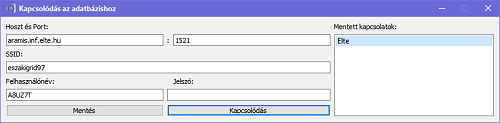
\includegraphics[max width=\textwidth]{connect}
  \end{center}
 \caption{Kapcsolódási ablak}
\end{figure}
A mentett kapcsolatok kezelésére itt is lehetőség van.
Duplán kattintva egy kapcsolat nevére betölthetjük annak adatait. Ha valamelyik mező üresen lett hagyva,
akkor az ablakban levő mező is üres lesz. (Abban az esetben is, ha korábban lett bele írva.)
A \textit{delete} billentyű lenyomására a kijelölt kapcsolat törlődik, de
mielőtt véglegesen törölné a program kér egy megerősítést a felhasználótól.
Lehetőség van az aktuális, képernyőn látható kapcsolati adatok mentésére is. Ekkor egy nevet kell megadni a kapcsolatnak, ami nem lehet üres,
valamint két különböző kapcsolat nem szerepelhet ugyanazon névvel, ennek ellenére felül lehet írni jelenleg létező kapcsolatot ha módosítani
kívánjuk.
Az adatok helyes megadása után, illetve ha létrejön sikeresen a kapcsolat az adatbázissal, akkor a program beléptet a fő ablakhoz.
Hiba esetén kiírja a hibakódot, ezekről részletesebben 2.3-as szakaszban olvashat.

\section{A kapcsolódási ablaknál előforduló hibák}

\begin{figure}[ht]
  \begin{center}
  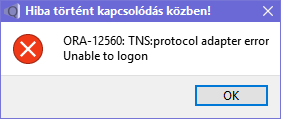
\includegraphics[max width=\textwidth]{database_error}
  \end{center}
 \caption{Kapcsolódási hibára példa}
\end{figure}

Kapcsolódás közben több hiba is előfordulhat, csakhogy ezeket az adatbázis szerver kezeli, nem a DiagramQuery.
Néhány gyakori hibát megemlítenék, ami hasznos lehet
a program első használata során. A következő hibakódok fordulhatnak elő a leggyakrabban:
\begin{itemize}
  \item \textbf{ORA-12560}: TNS:protocol adapter error; Unable to logon. Ezt okozhatja internetkapcsolat hiánya,
  vagy hiányzó szervernév, azaz ha nem lehet kiépíteni kapcsolatot a szerverrel bármilyen okból.
  \item \textbf{ORA-01005}: null password given; logon denied; Unable to logon. Ezt a hibaüzenetet akkor fogja kapni,
  ha a jelszó mezőt üresen hagyja. (Ha üres a jelszó mező akkor hibás felhasználónév esetén is ez a hibaüzenet jön elő)
  \item \textbf{ORA-01017}: invalid username/password; logon denied; Unable to logon. Hibás felhasználónév vagy jelszó 
  esetén jelenik meg ez a hibaüzenet.
\end{itemize}

Ezek a hibakódok természetesen más esetben is előjöhetnek, ha biztos benne hogy minden rendben van az adatokkal, és a
kapcsolattal, akkor kérjen meg egy hozzáértőt a probléma elhárításában (mivel ebben az esetben nagy valószínűséggel
magával az adatbázis szerverrel van probléma).

Az Oracle Docs\cite{oracledocs} oldalán megtalálható minden hibakód, és a hibák okai (angolul).
Legtöbb esetben elég beszédesek, így meg lehet őket érteni dokumentáció nélkül is, valamint ha magyar nyelvű
\textit{Oracle Instantclient}-et tölt le, abban az esetben magyarul jelennek meg a hibaüzenetek magyarázatai.
A későbbiekben is ezen hibakódok vannak használva (és logolva), így ezt az oldalt érdemes a későbbiekben is látogatni.

A továbbiakban a kapcsolódási ablak saját hibaüzeneteit részletezném:
\begin{itemize}
  \item \textbf{Kapcsolat törlése sikertelen!}: Ez akkor fordulhat elő, ha nincs joga ahhoz a fájlhoz ami
  ezt a kapcsolatot tartalmazza, vagy abban az esetben ha futás közben már törölve lett.
  \item \textbf{Kérem ellenőrizze jogosultságát a program könyvtárához.}: A program a Connections nevű mappát
  próbálja létrehozni abban az esetben, ha nem létezik, és ez a hibaüzenet fog megjelenni akkor, ha ez a kísérlet meghiúsul.
  \item \textbf{Kérem adjon meg egy nevet, amivel később majd el lehet érni a kapcsolatot!}: akkor jelenik meg, hogyha üres
  szöveget próbált megadni a kapcsolat nevének.
  \item \textbf{Fájl megnyitása sikertelen!}: akkor jelenik meg, ha mentés közben a program nem fér hozzá a
  Connections/\textbf{$<$kapcsolatneve$>$}.xml fájlhoz.
\end{itemize}

\newpage

\section{Grafikus felület}
\begin{figure}[ht]
    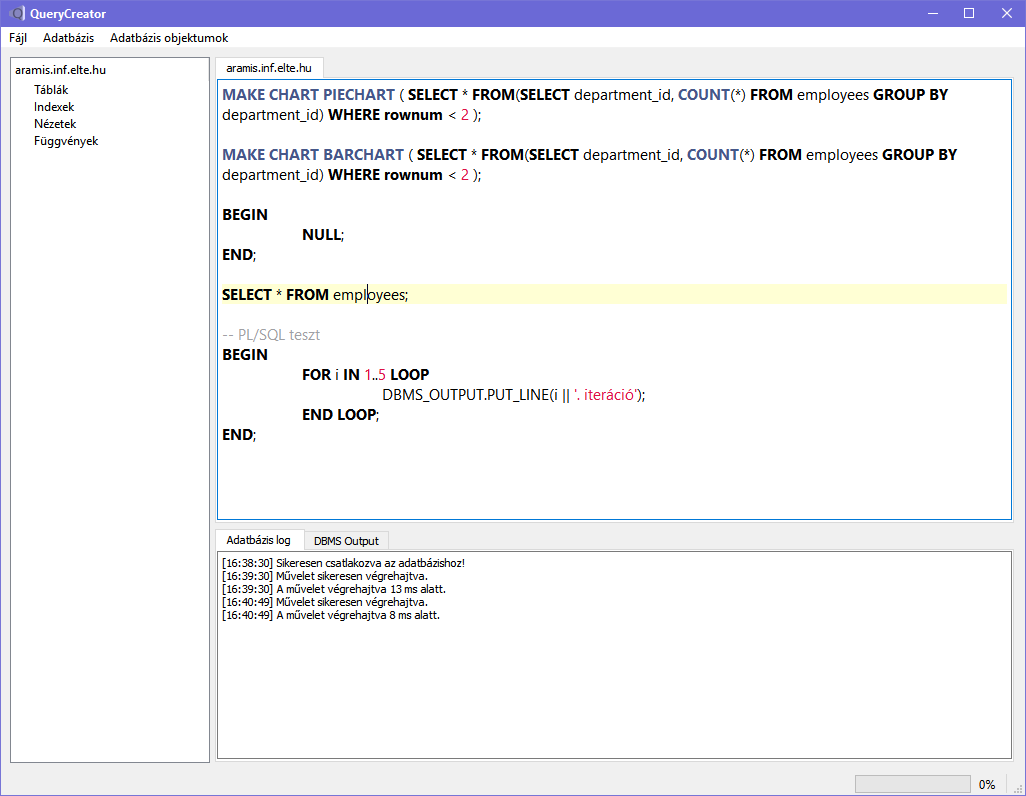
\includegraphics[width=1.0\textwidth]{gui}
 \caption{Felhasználói felület}
\end{figure}
Sikeres belépés esetén egy ehhez hasonló képernyő fogadja a felhasználókat.
A következő billentyűparancsok használhatóak az ablakon belül:
\begin{itemize}
  \item \textbf{CTRL+W, illetve CTRL+SHIFT+W}: bezárja alsó, illetve felső lapot. Az alapértelmezett lapokat nem lehet bezárni.
  \item \textbf{CTRL+ENTER}: A szerkesztőben lévő lekérdezést vagy szkriptet végrehajtja kurzor helyzetétől függően.
  \item \textbf{F4}: Lekérdezési terv létrehozása.
  \item \textbf{F3}: Kijelölt utasítás(ok) végrehajtása.
  \item \textbf{DELETE}: Adatbázis objektum törlése a bal oldali fából.
\end{itemize}

Ezeket a parancsokat nem csak billentyűkombinációk révén lehet elérni, hanem kattintással, illetve menüből is elérhetőek.

A menüben lévő parancsokról röviden:
\begin{itemize}
  \item \textbf{Fájl $\rightarrow$ Új} - Új lapot hoz létre a program, azaz töröl minden szöveget a jelenlegi szerkesztőből. Mielőtt ezt megtenné,
természetesen figyelmezteti erről a felhasználót. CTRL + N billentyűkombinációval is elérhető.
  \item \textbf{Fájl $\rightarrow$ Megnyitás...} - Törli a jelenlegi lap tartalmát és betölti a kiválasztott fájlt. Hiba vagy visszalépés esetén
  megmarad a korábban írt lap tartalma. CTRL + O billentyűkombinációval is elérhető.
  \item \textbf{Fájl $\rightarrow$ Mentés másként...} - Elmenti a jelenlegi lap tartalmát. Hiba esetén jelez, és nem történik mentés.
  CTRL + S billentyűkombinációval is elérhető.
  \item \textbf{Fájl $\rightarrow$ Kilépés} - Kilépés a programból. A nem mentett munka elveszik, a program nem figyelmeztet nem mentett tranzakciókról,
  se a szerkesztőbe írt, de nem mentett adatokról, azonban megerősítést kér, mielőtt kilép. CTRL + Q billentyűkombinációval is elérhető.
  \item \textbf{Szerkesztés $\rightarrow$ Parancs futtatása} - Ugyan az a hatás érhető el vele, mint a \textit{CTRL+ENTER} billentyűkombinációval.
  \item \textbf{Szerkesztés $\rightarrow$ Kijelölés futtatása} - \textit{F3}-hoz hasonlóan végrehajta a kijelölt utasítást.
  \item \textbf{Szerkesztés $\rightarrow$ Lekérdezési terv megjelenítése} - Nem különb a hatása, mint az \textit{F4} megnyomásának: a kurzor helyén lévő lekérdezéshez,
  vagy a kijelölt lekérdezéshez készít lekérdezési tervet, majd jeleníti meg azt.
  \item \textbf{Adatbázis $\rightarrow$ Újrakapcsolódás...} - Megpróbál új kapcsolatot kiépíteni az adatbázis szerverrel. Az újrakapcsolódáshoz meg kell adnia ismét
  a jelszavát.
  \item \textbf{Adatbázis $\rightarrow$ Új kapcsolat} - Bontja a jelenlegi kapcsolatot a felhasználó beleegyezése után, és nyit egy új kapcsolódási ablakot.
  \item \textbf{Adatbázis objektumok $\rightarrow$ Megtekintés} - Az adatbázis objektumok fájában jelenleg kijelölt objektum tulajdonságairól megnyit egy új lapot.
  \item \textbf{Adatbázis objektumok $\rightarrow$ Törlés} - A jelenleg kijelölt adatbázis objektumot törli beleegyezés után.
\end{itemize}

Itt még egy dologra felhívnám a figyelmet: Ha időtúllépés miatt kiléptet az adatbázis (ezt az adatbázis szerver beállításaitól függ mennyi idő), akkor
érdemes az újrakapcsolódást választani, mivel ha lekérdezést próbál végrehajtani, akkor az adatbázis sokáig nem fog válaszolni.

Az ablak bal oldalán található az adatbázis objektumok fája. Dupla kattintás esetén betöltődnek ezek az objektumok, majd ezután lehetőség nyílik ezek megtekintésére
(dupla kattintás), illetve törlésére (\textit{delete} billentyű). Ismételt dupla kattintásra frissítésre kerülnek az adatok. Táblák megtekintése esetén előjön az
attribútumainak neve, típusa, hossza, illetve hogy lehet-e az adott attribútum null. Indexeknél megtekinthető az index típusa, az hogy melyik táblához készült az index, illetve
ennek a táblának a tulajdonosa, továbbá az hogy egyedi-e az index. Nézeteknél meg lehet nézni a lekérdezést amivel a nézet létre lett hozva, a nézet típusát, illetve
hogy csak olvasható-e az adott nézet. Függvényeknél a függvény neve, id-ja, illetve létrehozási dátuma tekinthető meg. Ezt a fát igény esetén el is lehet tüntetni,
és akármikor vissza is lehet hozni. Ez hasznos lehet zavartalan íráshoz, vagy diagramok nagy méretben való megtekintésére.

A jobb alsó sarokban találhatóak az Adatbázis logja illetve kimenete, ezen felül ide kerülnek a végrehajtott lekérdezések, és végrehajtási tervek is. Az adatbázis minden
sikertelen műveletet logol a hiba okával együtt, illetve a sikeres műveleteket is, a végrehajtáshoz szükséges idővel együtt. Ez a log (ha sikeresen létrehozható) megtalálható
lesz később a háttértáron is, \textit{Logs} mappában \textit{ev\_honap\_nap.log} formában. Ha nem lépünk ki a programból a nap váltása előtt, akkor előző napi loghoz fog írni. Az adatbázis
kimenete minden esetben működik, nincs szükség külön parancs beírására hogy megjelenítsük azt. Mindemellett ez a komponens is eltüntethető, abban az esetben ha a felhasználó számára éppen nem
szükséges.

\subsection{Lekérdezések}

\begin{figure}[ht]
  \begin{center}
  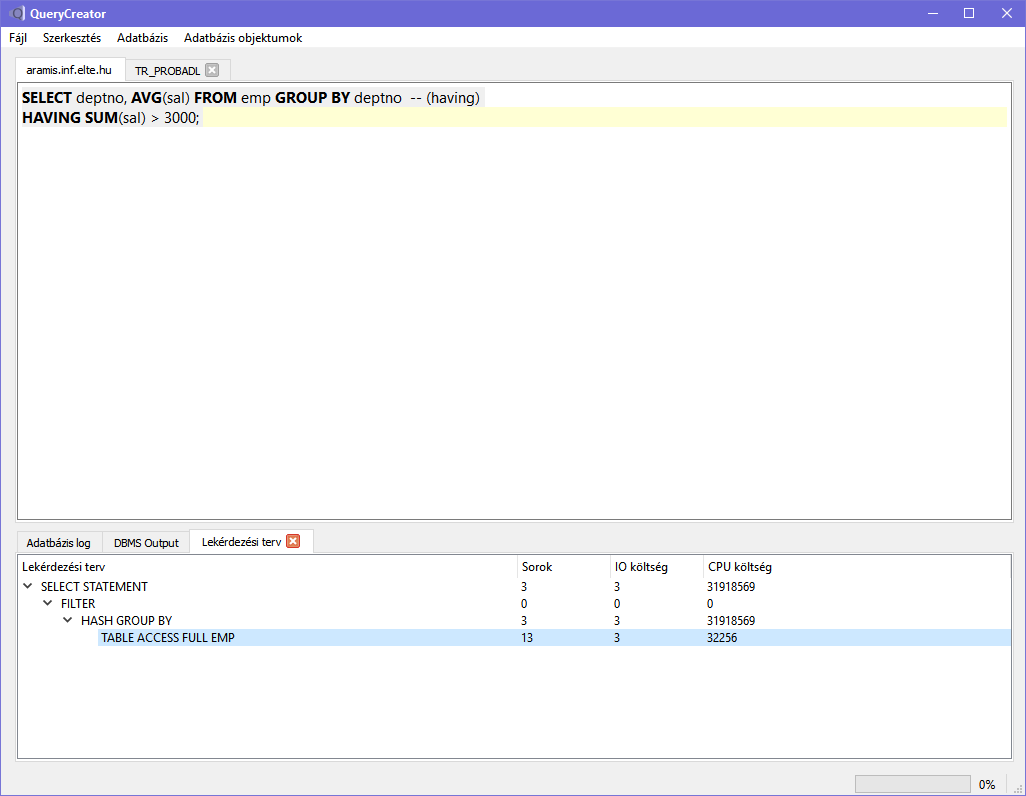
\includegraphics[max width=\textwidth]{expl_plan}
  \end{center}
 \caption{Lekérdezési terv megtekintése}
\end{figure}

A program szerkesztő felületében lehetőség van SQL lekérdezések, illetve PL/SQL szkriptek végrehajtására. SQL* Plus szkriptek viszont
nem működnek, így olyan utasításokat mint a \textbf{set serveroutput on} nem hajthatunk végre, csakhogy erre nincs is szükség, az adatbázis kimenet alapértelmezetten
használható. A programban szintaxis kiemeléssel jelennek meg ezek az utasítások, így tanulás közben is használható. Azonban szemantikus elemzés és automatikus
kitöltés nincsen a programban. Az SQL parancsokat érdemes pontosvesszővel elválasztani, ennek ellenére nem kötelező, pontosvessző hiányában is végrehajthatóak.
Nincs szükség PL/SQL parancsok lezárására '/' karakterrel mint SQLDeveloper esetén.

\subsection{Diagramok}
Két különböző típusú diagram lett implementálva a programban, a kör- és oszlopdiagram. A továbbiakban
ezeknek a szintaxisát részletezem, illetve leírom mikre használhatóak, mivel ezek különböző adatok
reprezentációjára alkalmasak.

\subsubsection{Kördiagram}
\begin{figure}[ht]
  \begin{center}
    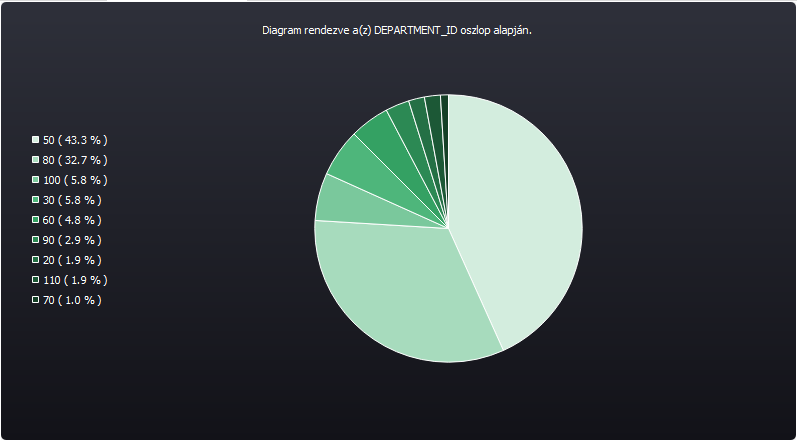
\includegraphics[width=1.0\textwidth]{piechart}
  \end{center}
 \caption{Kördiagram}
\end{figure}

A kördiagram kategorikus adatok megjelenítésére használható, azaz egy adott mennyiség megoszlásának arányát lehet vele
ábrázolni. Erre láthatunk egy példát a 2.5-ös ábrán. A kört akkora részekre osztjuk, amekkora részt az adott mennyiségek kitesznek az egészből. Akkor érdemes ezt
a fajta diagramot használni, ha egyes részeknek az egészhez való viszonyát kívánjuk megvizsgálni. Lehetőség lenne egy-egy
körcikket kirobbantani, azonban ez zavarólag hathat, így erre jelenleg nincs lehetőség a programban. Többet olvashat erről a
Számítógépes adatfeldolgozás\cite{szamadat} című könyvben, ami az interneten is elérhető.

Szintaxisa a következő:

\textbf{{\color{awesomeblue} MAKE CHART PIECHART }} ( \textbf{$<$SQL lekérdezés$>$} );

\textbf{Az SQL lekérdezésnek ezeket a feltételeket kell teljesítenie:}
\begin{itemize}
  \item A lekérdezés nem lehet üres.
  \item Legalább kettő, legfeljebb húsz rekordos lehet a lekérdezés.
  \item Két attribútumosnak kell lennie a lekérdezésnek.
  \item Második attribútuma lehet egy aggregáló függvény eredménye, vagy egy természetes szám. 
  Negatív szám nem használható, hiszen ebben a kontextusban értelmetlen.
  \item Érdemes csökkenő sorrendben lekérni az elemeket, de ez teljes mértékben a felhasználóra van bízva.
  \item Felesleges attribútum nem szerepelhet a lekérdezésben, azaz ha kettőnél többet tartalmaz, akkor hibát fog adni a program.
\end{itemize}

A címkékben százalékosan jelennek meg az adatok, így érdemes lehet úgy lekérni az adatokat, hogy ne történjen hiba
a kerekítés során.
\newpage
\subsubsection{Oszlopdiagram}
\begin{figure}[ht]
  \begin{center}
    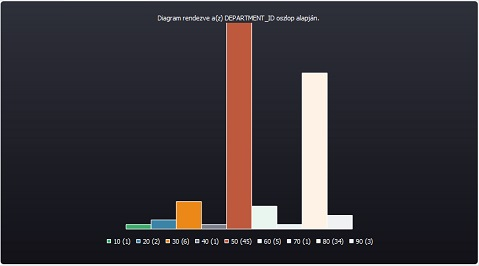
\includegraphics[width=1.0\textwidth]{barchart}
  \end{center}
 \caption{Oszlopdiagram}
\end{figure}

Az oszlopdiagram különböző, ennek ellenére egynemű, időszakosan változó adatok megjelenítésére használható. Erről a típusról láthat egy példát a
2.6-os ábrán. Ez lehet például egy
bolt napi nyeresége, ami természetesen nem feltétlen pozitív minden nap, így szükség lehet negatív számok megjelenítése is. Az adatok
változása így könnyen leolvasható, és összehasonlítható lesz. Erről a diagramtípusról bővebben olvashat Nyesőné Marton Mária
könyvében\cite{szamadat}.

Szintaxisa a következő:

\textbf{{\color{awesomeblue} MAKE CHART BARCHART }} ( \textbf{$<$SQL lekérdezés$>$} );

\textbf{Az SQL lekérdezésnek ezeket a feltételeket kell teljesítenie:}
\begin{itemize}
  \item A lekérdezés nem lehet üres.
  \item Legalább kettő, legfeljebb tíz rekordot tartalmazhat.
  \item Két attribútumosnak kell lennie a lekérdezésnek.
  \item Második attribútuma lehet egy aggregáló függvény eredménye, vagy egy egész szám.
  \item Felesleges attribútum nem szerepelhet a lekérdezésben, azaz ha kettőnél többet tartalmaz hibát fog adni a program.
\end{itemize}

Érdemes eredeti sorrendben meghagyni az adatokat, hogy könnyen megfigyelhessük a kiugró adatokat.

\section{Hibák a fő ablaknál}

\begin{figure}[ht]
  \begin{center}
  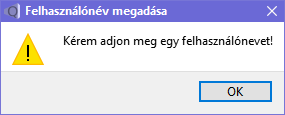
\includegraphics[max width=\textwidth]{username_missing}
  \end{center}
 \caption{Újrakapcsolódás közben fellépő hibára példa}
\end{figure}

Számtalan hiba fordulhat elő fő ablak használata közben, ennek ellenére a felugró hibák száma elenyésző.
Röviden most ezeket, és ezeknek a magyarázatát sorolnám fel:

\begin{itemize}
  \item \textbf{Kérem adjon meg egy felhasználónevet!}: akkor jelenik meg, ha újracsatlakozásnál nem adott meg
  egy felhasználónevet se. A program automatikusan beírja a jelenleg kapcsolódott felhasználót, csakhogy lehetőség van más felhasználóval való
  belépésre is.
  \item \textbf{Kérem adja meg jelszavát!}: abban az esetben jelenik meg, ha újrakapcsolódásnál nem adott meg jelszót.
  \item \textbf{Sikertelen kapcsolódás}: akkor, ha valamilyen okból (internetkapcsolat megszűnt, hibás felhasználónév/jelszó páros) nem sikerült
  újra kiépíteni a kapcsolatot az adatbázissal. Egy hibaüzenet is megjelenik, ami a korábban említett Oracle oldalán\cite{oracledocs} megtekinthető.
\end{itemize}

Az utasítások futtatása során azonban ennél jóval többféle hibaüzenet is megjelenhet. Az alábbi üzenetek az adatbázis logjában találhatóak meg, ezek később is visszanézhetőek.
Ezeknek a nagy részét lefedi az Oracle oldala\cite{oracledocs}, csakhogy
vannak a programnak saját hibaüzenetei is, ezeket részletezném:

\begin{itemize}
  \item \textbf{Kérem hozza létre a PLAN\_TABLE táblát ezen parancs használata előtt!} - a lekérdezési terv létrehozásához szükséges egy PLAN\_TABLE nevű tábla,
  erről bővebben az Oracle dokumentációjában\cite{oracledocsref} olvashat.
  \item \textbf{Hiba: üres lekérdezést próbált végrehajtani!} - ha kijelölést próbál végrehajtani, de nincs semmi kijelölve, akkor kapja ezt a hibaüzenetet. Illetve ha
  nincs semmi a szerkesztőablakba, és akkor próbál egy utasítást végrehajtani.
  \item \textbf{Nem GROUP BY lekérdezés.} - ez a hibaüzenet akkor jelenik meg, ha megpróbált egy diagramout létrehozni olyan lekérdezéssel, amelyben nem szerepel \textbf{group by}.
  \item \textbf{A diagram működéséhez 2 oszlop szükséges.} - akkor jelenik ez meg ha kettőnél kevesebb, vagy több attribútumu lekérdezéssel próbál egy diagramot létrehozni.
\end{itemize}

\begin{figure}[ht]
  \begin{center}
  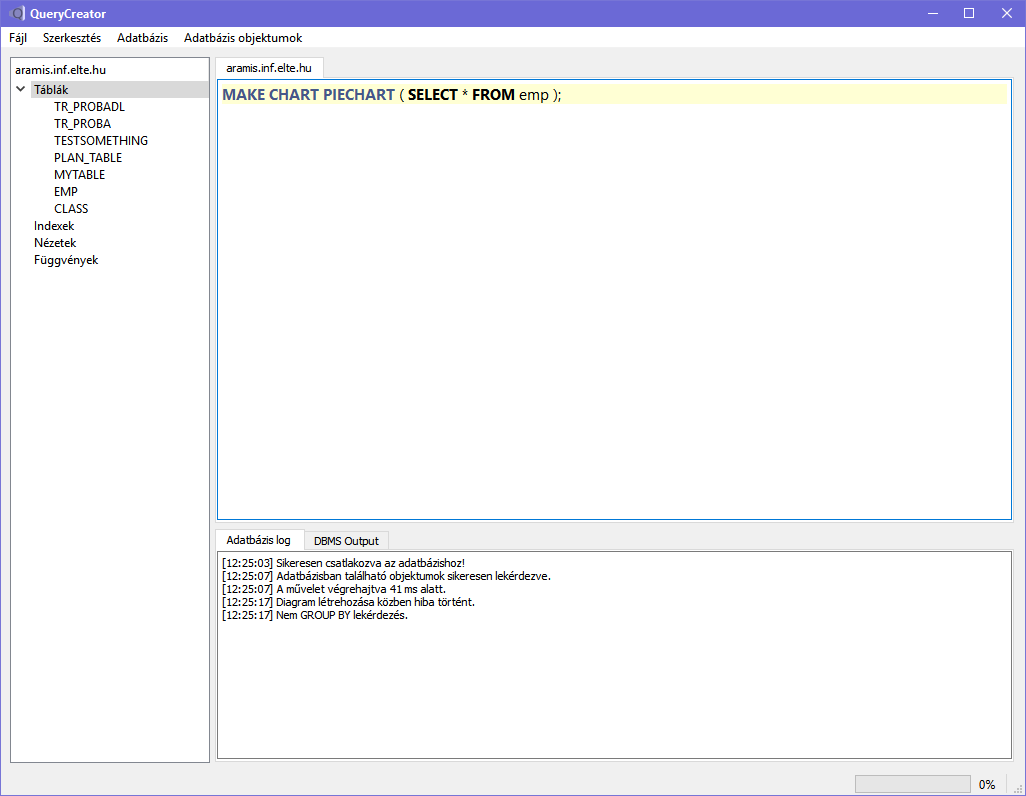
\includegraphics[max width=\textwidth]{error_diagram}
  \end{center}
 \caption{Diagram létrehozása közben fellépő hiba}
\end{figure}

\begin{itemize}
  \item \textbf{Második oszlopnak számot kell tartalmaznia!} - ha a felhasználó nem aggregációs lekérdezést használ, vagy olyan oszlopot ad meg második attribútumként ami nem egy
  szám, akkor ez a hibaüzenet fogadja.
  \item \textbf{Kérem kördiagramot csak pozitív számokkal használjon!} - mivel a kördiagram adatok egymáshoz való viszonyítását szemlélteti, és az egyes adatok százalékban jelennek meg
  az egészhez viszonyítva, így nem lenne értelme negatív számokkal használni azt. Ez a hibaüzenet erre a hibára figyelmeztet.
  \item \textbf{Nem támogatott diagram típus: <diagramtípus>} - ez az üzenet akkor jelenik meg ha egy nem támogatott diagramtípust próbál létrehozni.
  Jelenleg támogatott típusok: piechart, barchart.
  \item \textbf{Kérem ezt a diagramtípust kevesebb rekorddal használja.} - abban az esetben ha túl sok rekorddal rendelkező lekérdezéssel próbál egy diagramot készíteni, akkor
  fog ezzel a hibaüzenettel találkozni. Kördiagram esetén húsz, míg oszlopdiagram esetén tíz a maximális rekordszám.
  \item \textbf{Üres lekérdezés.} - amennyiben egy rekorddal se rendelkezik a lekérdezés amivel a diagramot próbálja létrehozni, akkor ez az üzenet fogadja.
\end{itemize}

Ezeknek a hibaüzeneteknek nagy része elkerülhető ha körültekintően hozza létre a diagramokat, illetve hajtja végre a lekérdezéseket. Mielőtt használná a programot
érdemes elolvasni a 2.3.2-es szakaszban lévő leírást a diagramok használatáról, illetve hasznukról.

DiagramQuery arról is figyelmeztet, hogy ha egy törlés / megtekintés / lekérdezés nem sikerül, és ezen felül az Oracle saját hibakódját is megjeleníti, így pontosan
meg lehet tudni milyen hiba történt az utasítás végrehajtása során.


\begin{enumerate}
  \item beállításaitól
  \item kapcsolat
  \item given
  \item magyar
\end{enumerate}